\section{Laplacetransformation}
Mittels der Laplacetransforamtion können kausale Signale analysiert werden. Sollte das Signal nicht kausal sein wird es mit der Einschaltfunktion multipliziert.\\
\begin{tabular}{c}
	$F(s)=\int\limits_0^\infty f(t)e^{-st}dt \qquad s=\sigma+j\omega$\\
	$Originalbereich \;\laplace\; Bildbereich$\\
\end{tabular}

\subsection{Eigenschaften der Laplacetransformation}
\begin{tabular}{|l|l|}
	\hline
	Linearität & 
	$\alpha\cdot f(t) + \beta\cdot g(t) \;\laplace\; \alpha\cdot F(s) + \beta\cdot
	G(s)$ \\
	\hline
	Zeitskalierung &
	$f(\alpha t) \;\laplace\; \frac{1}{\alpha}F \left (\frac{s}{\alpha} \right ) \quad 0
	<\alpha \in\mathbb{R}$ \\
	\hline
	Faltung im Zeitbereich &
	$f(t) \ast g(t) = \int\limits_{0}^{\infty} f(\tau)g(t-\tau)d\tau \;\laplace\; F(s)
	\cdot G(s)$\\
	\hline
	Faltung im Frequenzbereich &
	$f(t) \cdot g(t) \;\laplace\; \frac{1}{2\pi j}\int\limits_{c-j\infty}^{c+j\infty}
	F(\xi) G(s-\xi)d\xi$ \\
	\hline
	Ableitung im Zeitbereich &
	$\frac{\partial f(t)}{\partial t} \;\laplace\; sF(s)
	-f(0+)$ \\
	\hline
	Ableitungen im Zeitbereich &
	$\frac{\partial^n f(t)}{\partial t^n} \;\laplace\; s^nF(s)
	-s^{n-1}f(0+)-s^{n-2}\frac{\partial f(0+)}{\partial t}-\ldots
	-s^0\frac{\partial^{n-1} f(0+)}{\partial t^{n-1}}$ \\
	\hline
	Multiplikation mit $t$ &
	$t\cdot f(t)  \;\laplace\; \frac{-\partial F(s)}{\partial s}$ \\
	\hline
	Ableitung im Frequenzbereich &
	$(-t)^n f(t) \;\laplace\;  \frac{\partial^n F(s)}{\partial s^n}$ \\
	\hline
	Verschiebung im Zeitbereich &
	$f(t\pm t_0) \;\laplace\; F(s)e^{\pm t_0 s}$ \\
	\hline
	Verschiebung im Frequenzbereich &
	$f(t)e^{\mp\alpha t} \;\laplace\; F(s\pm\alpha)$ \\
	\hline
	Integration &
	$\int\limits_0^t f(\tau)d\tau \;\laplace\; \frac{F(s)}{s}$ \\
	\hline
	Anfangswert &
	$\lim_{t\rightarrow 0} f(t) = \lim_{s\rightarrow \infty} sF(s),\text{~wenn
	}  \lim_{t\rightarrow 0} f(t)\text{~existiert}.$ \\
	\hline
	Endwert &
	$\lim_{t\rightarrow \infty} f(t) = \lim_{s\rightarrow 0} sF(s),\text{~wenn
	}  \lim_{t\rightarrow \infty} f(t)\text{~existiert}.$ \\
	\hline
\end{tabular}
\newpage
\subsection{Rücktransformation}
\subsubsection{Vorgehen}
\begin{minipage}{12cm}
	\begin{enumerate}
		\item Benutzung einer Tabelle zugehöriger Original-, und Bildfunktionen (Korrespondenzen)
		\item Umformen (Kürzen, Erweitern, etc.) um auf Korrespondenz zu schliessen
		\item Mittels Partialbruchzerlegung auf Korrespondenz schliessen
	\end{enumerate}
\end{minipage}
\begin{minipage}{7cm}
	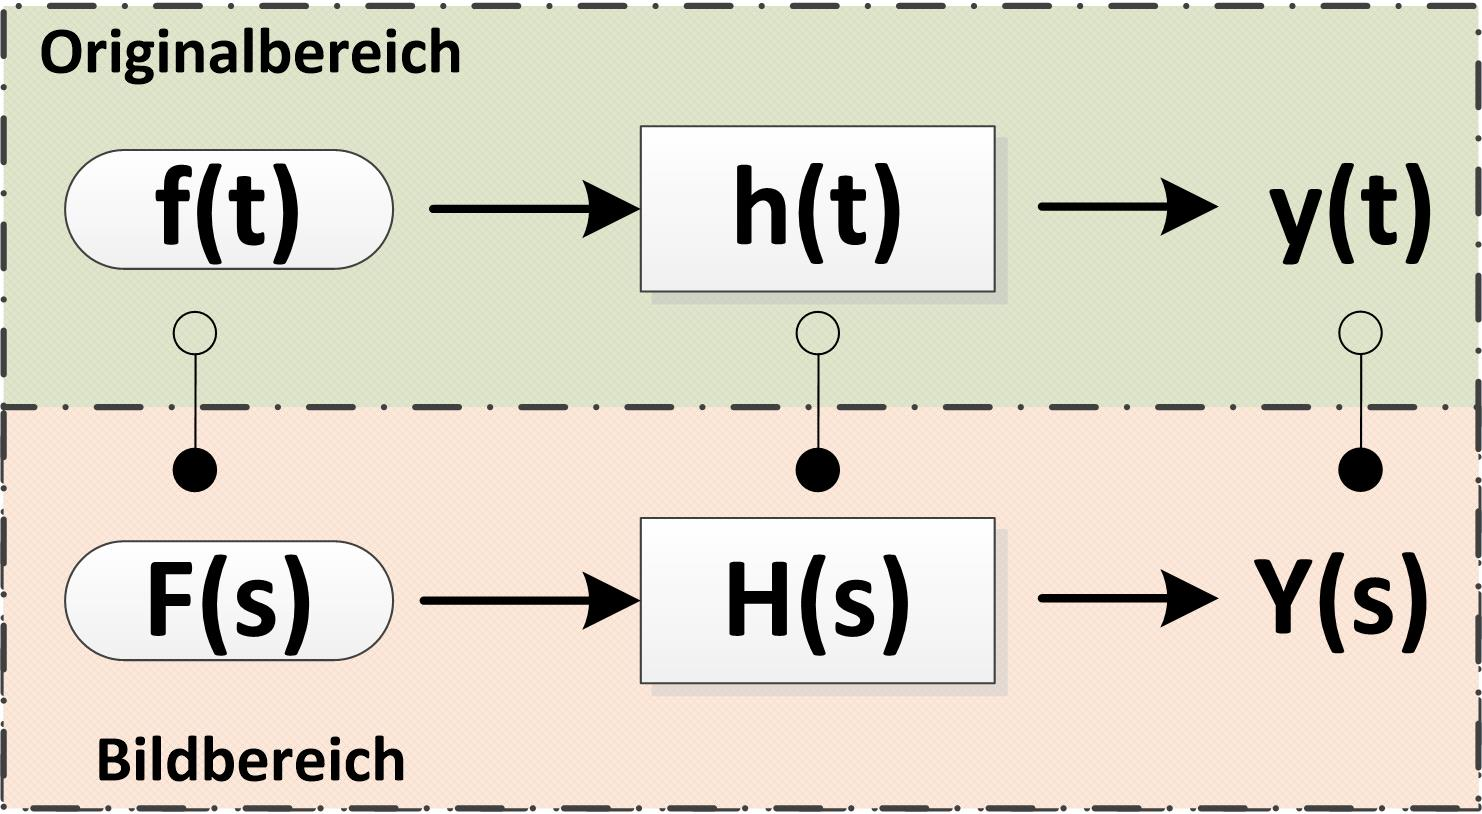
\includegraphics[width=7cm]{images/IntTra.jpg}
\end{minipage}

\subsubsection{Laplacetabelle}
\begin{multicols}{2}
	\begin{center}
		\begin{tabular}{|lcc|}
			\hline
			$\sigma \left( t \right)$ & $\; \laplace \;$ & $\frac{1}{s}$ \\
			$\sigma \left( t \right) \cdot t$ & $\; \laplace \;$ & $\frac{1}{s^2}$\\
			$\sigma \left( t \right) \cdot t^2$ & $\; \laplace \;$ & $\frac{2}{s^3}$\\
			$\sigma \left( t \right) \cdot t^n$ & $\; \laplace \;$ & $\frac{n!}{s^{n+1}}$\\
			$\sigma \left( t \right) \cdot e^{\alpha t}$ & $\; \laplace \;$ &
			$\frac{1}{s-\alpha}$\\
			$\sigma \left( t \right) \cdot t \cdot e^{\alpha t}$ & $\; \laplace \;$ &
			$\frac{1}{( s - \alpha )^2}$\\
			\hline
		\end{tabular}
	\end{center}
	\columnbreak
	\begin{center}
		\begin{tabular}{|lcc|}
			\hline
			$\sigma \left( t \right)\cdot t^2 \cdot e^{\alpha t}$ &
			$\; \laplace \;$ & $\frac{2}{{( s - \alpha )}^3}$\\
			$\sigma \left( t \right)\cdot t^n \cdot e^{ \alpha t}$ &
			$\; \laplace \;$ & $\frac{n!}{(s-\alpha)^{n+1}}$\\
			$\sigma \left( t \right) \cdot \sin \left(\omega t \right)$ & $\; \laplace \;$ &
			$\frac{\omega}{s^2 + {\omega^2}}$\\
			$\sigma \left( t \right) \cdot \cos \left( \omega t \right)$ & $\; \laplace \;$ &
			$\frac{s}{ s^2 + \omega^2}$\\
			$\delta \left( t \right)$ & $\; \laplace \;$ & $1\left( s \right)$ \\
			$\delta \left( t - \alpha \right)$ & $\; \laplace \;$ & $e^{- \alpha s}$\\
			\hline
		\end{tabular}
	\end{center}
\end{multicols}

\subsection{Lösen von Differentialgleichungen mit Laplace}
\begin{minipage}{11.5cm}
	\begin{tabular}{| l | l |}
		\hline
		Übertragungsfunktion & $G(s) = \frac{1}{p(s)} \quad g(t) \; \laplace \; G(s)$\\
		\hline Charakteristisches Polynom & $p(s)$\\
		\hline
		Frequenzgang & $G(j\omega) = H(\omega)$ \\
		\hline
		Impulsantwort & $y_{\delta}(t) = g(t) = y_{\sigma}'(t) \; \laplace \; G(s) = \frac{1}{p(s)}=Y_{\delta}(s)$\\
		\hline
		Sprungwantwort & $y_{\sigma}(t)=\int\limits_0^t g(u) du \; \laplace \; \frac{G(s)}{s} = \frac{1}{s \cdot p(s)} = Y_{\sigma}(s)$\\
		\hline
		Eigenschwingung & $\frac{h(s)}{p(s)}$ \\
		\hline
		äussere Erregung & $\frac{F(s)}{p(s)}$ \\
		\hline
		stationärer Zustand & = ungedämpfte Eigenschwingung\\
		\hline
	\end{tabular}
\end{minipage}
\newpage
\subsubsection{Lineare DGL mit Anfangswerten}
Gegeben sei eine Differentialgleichung mit Anfangsbedingungen.Sind keine Anfangsbedingungen vorhanden können die daraus entstehenden Terme vernachlässigt werden.\\
\vspace{2pt}
\begin{tabular}{l l}
	DGL & $a_n y^{n}(t)+a_n-1 y^{n-1}+...a_1 y'(t)+a_0 y(t)=f(t)$\\
	Endterm & $a_0\cdot[Y(s)]+a_1 \cdot [sY(s)-f(0)]+a_n-1y^n-1 \cdot [s^nY(s)-s^{n-1} \cdot f(0)-s^{n-2}f'(0)...-f^{n-1}(0)]=F(s)$\\
\end{tabular}

\begin{minipage}{15cm}
	$y(t) \; \laplace \;  Y(s)$\\
	$y'(t) \; \laplace \; sY(s) - f(0)$\\
	$y''(t) \; \laplace \; s^2Y(s)-s\cdot f(0) - f'(0)$\\
	$y'''(t) \; \laplace \; s^3Y(s)-s^2\cdot f(0)-s \cdot f'(0) - f''(0)$\\
	$y^n(t) \; \laplace \; s^nY(s)-s^{n-1}\cdot f(0)-s^{n-2} \cdot f'(0) ...- f^{n-1}(0)$\\
	$y^{(n)} \; \laplace \; 
	\underbrace{s^nY(s)}_{Y(s) \cdot p(s)}
	\underbrace{-s^{n-1}y_0 - \dots - y^{(n-1)}}_{h(s)}$\\
\end{minipage}
\includepdf[pages={8-9},pagecommand={},,scale=0.98]{sections/Tabellen.pdf}
\clearpage
\pagebreak